\documentclass[12pt]{report}
\usepackage[spanish]{babel}
\usepackage[utf8]{inputenc}
\usepackage{graphicx}
\usepackage{verbatim}
\usepackage{listings}
\usepackage{float}
\renewcommand*\thesection{\arabic{section}}

\begin{document}
	
	\begin{center}
		\textbf{Análisis de Algoritmos, Sem: 2018-1, 3CV1, Práctica 4, 09-2017}
		\newline
	\end{center}
	
	\begin{center}
		\begin{picture}(0,0) \put(-125,-55){
			\includegraphics[width=2.7cm]{../../IPNlogo.jpg}} 
		\end{picture}
		\LARGE Escuela Superior de Cómputo.\\
		Instituto Politécnico Nacional, México.\\
		\begin{picture}(0,0) \put(160,10){
			\includegraphics[width=2.7cm]{../../logoescom.png}} 
		\end{picture}
	\end{center}
	
	\begin{center}
		\Large Práctica 4: Divide y Vencerás: QuickSort.\\
	\end{center}
	
	\begin{center}
		\textbf{Blancas Pérez Bryan Israel}\\
		orionmunecaycanica@gmail.com\\
	\end{center}
	
	
	\textbf{\large Resumen: }Aplicar la técnica "Divide y Vencerás" con el algoritmo de ordenamiento QuickSort, y encontrar el orden de complejidad en diferentes casos.\newline\\
	
	\textbf{\large Palabras Clave: } Divide y Vencerás, Partition, QuickSort.\\
	

	\section{Introducción}
	En está práctica se implementará el algoritmo de ordenamiento QuickSort. Este algoritmo es conocido por ser uno de los más rápidos, sin embargo en esta práctica, veremos que el orden de complejidad es cambiante debido al algoritmo que usa el QuickSort para apoyarse, llamado "Partition".\newpage
	
	

	\section{Conceptos Básicos}
	\textbf{Partition.}\\
	
	Partition, es un algoritmo que divide un arreglo tamaño $n=p-r+1$ en dos arreglos de tamaños $q-p+1$ y $r-q$, de tal forma que $A[q]>A[i] \  \forall \ p \leq i <q$ y $A[q] < A[i] \ \forall \ q<i\leq r$.\\
	
	\textbf{QuickSort.}\\
	
	EL algoritmo QuickSort, es un algoritmo creado por el científico británico Hoare, basado en la técnica Divide y Vencerás [1]. EL algoritmo ordena de la siguiente forma:\newline \newline
	\textbf{1.} Se elige un elemento de la lista, llamado pivote.\newline
	\textbf{2.} Se acomoda la lista de tal forma que todos los números del lado izquierdo del pivote son menores a él, y todos los números del lado derecho del pivote, son mayores a él.\newline
	\textbf{3.} Al quedar la lista separada en dos sublistas, se repite el proceso de forma recursiva con cada una de ellas. Hasta que cada sublista sea de tamaño 1.\newline
	\textbf{4.} Una vez terminado este proceso, todos los elementos estarán ordenados.\\ 
	
		
	
	\section{Experimentación y Resultados}	
	\textbf{Ejercicio 1.}\\
	Implementar el algoritmo QuickSort.\newline
	
	\textbf{i) Mediante gráficas, muestre que el algoritmo Partition tiene orden de complejidad lineal.}\newline
	Pseudocódigo del algoritmo Partition:
	\lstset{language=C, breaklines=true, basicstyle=\footnotesize}
	\lstset{numbers=left, numberstyle=\tiny, stepnumber=1, numbersep=10pt}
	\begin{lstlisting}
Partition(a,p,r)
  x=a[r]
  j=p-1
  for i = p to r-1 do
    if a[i] < x then
      j++
      exchange(a[j],a[i])
  j++
  exchange(a[j],x)
  return j
	\end{lstlisting}
	
	El algoritmo Partition, recibe como entrada un arreglo $A[p,...,r]$. Primeramente, elige como pivote al último número del arreglo y sitúa dos indices i y j, i apuntando en el inicio del arreglo y j=i-1. Después, compara cada elemento del resto de números del arreglo con el pivote. Si el pivote es mayor al número en el que se está actualmente, se intercambia de posición los elementos en la posición j e i. Al final de este proceso, el arreglo a, queda dividido en dos subarreglos, separados por el pivote. Como salida, Partition devuelve la posición del pivote.\\
	
	\textbf{Gráfica de la función Partition\\}
	\begin{figure}[H]
		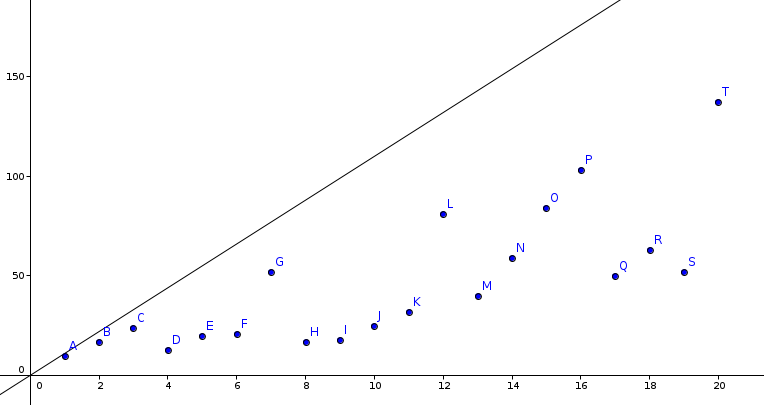
\includegraphics[width=15cm]{imagenes/1.png}
		\centering
		\caption{Ejecución del algoritmo Partition.}
		\centering
	\end{figure}
	En la figura 1, se observa como puntos azules a las ejecuciones del algoritmo ($n \ vs \ T(n)$). Como se puede observar existe una recta $y=11x$, la cual acota a los puntos, demostrando que el tiempo computacional del algoritmo puede variar para un mismo n, pero jamás superará su cota superior. \textbf{Por lo tanto el algoritmo Partition tiene orden lineal}.\newpage
	
	\textbf{ii) Demuestre analíticamente que el algoritmo Partition tiene orden de complejidad lineal.}\newline
	\begin{table}[htbp]
		\begin{center}
			\begin{tabular}{|l|l|}
				\hline
				\multicolumn{2}{|c|}{Análisis del Algoritmo Partition} \\ 
				\hline
				\textbf{Línea de Código} & \textbf{Orden de complejidad}\\
				\hline
				2 & $\theta (1)$ \\ \hline
				3 & $\theta (1)$ \\ \hline
				4 & $\theta (n)$ \\ \hline
				5 & $\theta (1)$ \\ \hline
				6 & $\theta (1)$ \\ \hline
				7 & $\theta (1)$ \\ \hline
				8 & $\theta (1)$ \\ \hline
				9 & $\theta (1)$ \\ \hline
				10 & $\theta (1)$ \\ \hline
			\end{tabular}
			\caption{Análisis del algoritmo.}
			\label{tabla:analisis}
		\end{center}
	\end{table}\\
	Aplicando el teorema de la suma, nos quedamos con el máximo orden de los bloques nivelados.\\ 
	
	$Por \ lo \ tanto \ T(n) \  \epsilon \ \theta (n).$\\
	
	\textbf{iii) Mediante gráficas, muestre que el algoritmo QuickSort complejidad $\theta (nlogn)$}. (Para obtener sus conclusiones, considere diferentes valores para un arreglo tamaño n).\\
	
	Pseudocódigo del algoritmo QuickSort:
	\lstset{language=C, breaklines=true, basicstyle=\footnotesize}
	\lstset{numbers=left, numberstyle=\tiny, stepnumber=1, numbersep=10pt}
	\begin{lstlisting}
QuickSort(a,p,q)
  if p < r then
    q = partition(a,p,r)
    QuickSort(a,p,q-1)
    QuickSort(a,q+1,r)
	\end{lstlisting}
	
	EL algoritmo QuickSort, recibe como parámetros de entrada, un arreglo $a$ con su inicio (p) y el fin (r). Lo que hace el algoritmo es verificar que el arreglo $a$ sea de tamaño mayor a uno; si se cumple esa condición, se llama a la función partition para que divida el arreglo en dos subarreglos y se vuelve a llamar a la función QuickSort, con p y r modificados, para que siga dividiendo el arreglo hasta que sea de tamaño uno.\\
	
	\textbf{Gráfica de la función QuickSort\\}
	\begin{figure}[H]
		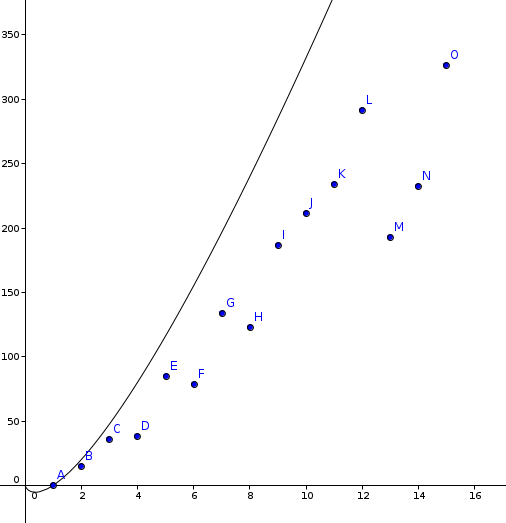
\includegraphics[width=10cm]{imagenes/2.png}
		\centering
		\caption{Ejecución del algoritmo QuickSort.}
		\centering
	\end{figure}
	En la figura 2, se observa como puntos azules a las ejecuciones del algoritmo ($n \ vs \ T(n)$). Como se puede observar existe una función $f(n) = 10n logn$, la cual acota a los puntos, demostrando que el tiempo computacional del algoritmo puede variar para un mismo n (pues depende el pivote que devuelva partition), pero jamás superará su cota superior. \textbf{Por lo tanto el algoritmo Partition tiene orden $nlogn$}.\newpage
	
	\textbf{iv) Demuestra analíticamente que el algoritmo QuickSort tiene complejidad $\theta (nlogn)$, cuando el pivote divide al arreglo por la mitad}.\\
	
	\begin{table}[htbp]
		\begin{center}
			\begin{tabular}{|l|l|}
				\hline
				\multicolumn{2}{|c|}{Análisis del Algoritmo QuickSort} \\ 
				\hline
				\textbf{Línea de Código} & \textbf{Orden de complejidad}\\
				\hline
				2 & $\theta (1)$ \\ \hline
				3 & $\theta (n)$ \\ \hline
				4 & $T (q)$ \\ \hline
				5 & $T(n-q)$ \\ \hline
			\end{tabular}
			\caption{Análisis del algoritmo.}
			\label{tabla:analisis2}
		\end{center}
	\end{table} 
	Entonces.\\
	$T(n)=T(q)+T(n-1)+\theta(n)$\\
	Supongamos que $q$ divide al arreglo por la mitad.\\
	$T(n)=2T(n/2)+\theta(n)$.\\
	Por los ejercicios hechos en clase.\\
	$T(n) \ \epsilon \ \theta(n)$
	
	
	\newpage
	
	\textbf{v) Mediante gráficas, proponga el orden de complejidad de QuickSort cuando todos los elementos del arreglo son distintos y están ordenados de forma decreciente.}\\
	
	Gráfica de la función QuickSort cuando sus elementos están ordenados de forma decreciente.\\
	\begin{figure}[H]
		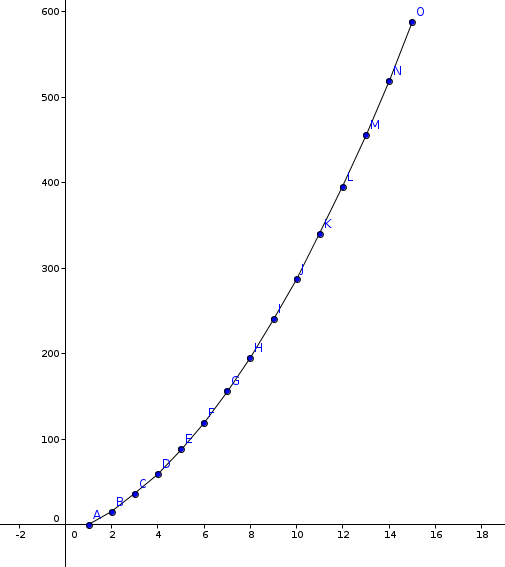
\includegraphics[height=9cm]{imagenes/3.png}
		\centering
		\caption{Ejecución del algoritmo QuickSort.}
		\centering
	\end{figure}
	En la figura 3, se observa la gráfica ($n \ vs \ T(n)$). Como se puede observar el comportamiento de la gráfica es distinto cuando todos los elementos del arreglo son distintos y están ordenados de manera decreciente. \textbf{Por lo tanto el orden de complejidad del algoritmo bajo estas condiciones es $T(n) \ \epsilon \ O(n^{2})$}.\newpage
	
\section{Conclusiones}
Esta práctica me pareció muy buena para darse cuenta de que no todos los algoritmos tiene un tiempo de ejecución constante. Es decir, QuickSort, como ya quedo demostrado, tiene un mejor y un peor caso. El mejor caso se da cuando el pivote termina en el centro de la lista de números, dando así un orden de complejidad de $nlogn$. Y su peor caso se da cuando los elementos están ordenados de manera decreciente, dando un orden de complejidad de $n^{2}$.\\
Sin duda esta práctica me gusto, por que además de todo, implementar el algoritmo tenia cierto grado de complejidad, ya que había que darse cuenta de pequeños casos que podrían impedir la buena ejecución del programa.\newpage 
	

\section{Anexo}

Resolver los siguientes problemas.\\

i) ¿Qué valor de q retorna Partition cuando todos los elementos en el arreglo A[p, ..., r] tienen el mismo valor?.\\

\textbf{R: 0}.\\

ii) ¿Cuál es el tiempo de ejecución de QuickSort cuando todos los elementos del arreglo tienen el mismo valor?\\

\textbf{R: el tiempo de ejecución se comporta de forma lineal.}

\section{Bibliografía}

[1] https://es.wikipedia.org/wiki/Quicksort\\
	
\end{document}